\documentclass[a4paper]{report}
\usepackage[utf8]{inputenc}
\usepackage[T1]{fontenc}
\usepackage{RJournal}
\usepackage{amsmath,amssymb,array}
\usepackage{booktabs}


% tightlist command for lists without linebreak
\providecommand{\tightlist}{%
  \setlength{\itemsep}{0pt}\setlength{\parskip}{0pt}}


% Always define CSL refs as bib entries are contained in separate doc
% Pandoc citation processing
\newlength{\cslhangindent}
\setlength{\cslhangindent}{1.5em}
\newlength{\csllabelwidth}
\setlength{\csllabelwidth}{3em}
\newlength{\cslentryspacingunit} % times entry-spacing
\setlength{\cslentryspacingunit}{\parskip}
% for Pandoc 2.8 to 2.10.1
\newenvironment{cslreferences}%
  {}%
  {\par}
% For Pandoc 2.11+
\newenvironment{CSLReferences}[2] % #1 hanging-ident, #2 entry spacing
 {% don't indent paragraphs
  \setlength{\parindent}{0pt}
  % turn on hanging indent if param 1 is 1
  \ifodd #1
  \let\oldpar\par
  \def\par{\hangindent=\cslhangindent\oldpar}
  \fi
  % set entry spacing
  \setlength{\parskip}{#2\cslentryspacingunit}
 }%
 {}
\usepackage{calc}
\newcommand{\CSLBlock}[1]{#1\hfill\break}
\newcommand{\CSLLeftMargin}[1]{\parbox[t]{\csllabelwidth}{#1}}
\newcommand{\CSLRightInline}[1]{\parbox[t]{\linewidth - \csllabelwidth}{#1}\break}
\newcommand{\CSLIndent}[1]{\hspace{\cslhangindent}#1}


\usepackage[most]{tcolorbox}
\usepackage{nameref}
\usepackage{booktabs}
\usepackage{bm, amsmath}
\usepackage{array}
\usepackage{multirow}
\usepackage{wrapfig}
\usepackage{float}
\usepackage{colortbl}
\usepackage{hhline}
\usepackage{xcolor}
\usepackage{longtable}
\usepackage{tabu}
\usepackage{adjustbox}
\usepackage{threeparttable}
\usepackage{makecell}
\def\greentick{
\includegraphics[scale=0.05]{figs/green_tick.png}}
\def\redcross{
\includegraphics[scale=0.05]{figs/red_cross.png}}
\newtcolorbox{blackbox}[1]{colback=white, colframe=black, coltext=black, boxsep=1.5pt, arc=4pt, before=\centering, title=#1}
\newenvironment{cols}[1][]{}{} \newenvironment{col}[1]{\begin{minipage}{#1}\ignorespaces}{\end{minipage} \ifhmode\unskip\fi
\aftergroup\useignorespacesandallpars} \def\useignorespacesandallpars#1\ignorespaces\fi{#1\fi\ignorespacesandallpars} \makeatletter
\def\ignorespacesandallpars{\@ifnextchar\par {\expandafter\ignorespacesandallpars\@gobble} {} } \makeatother

\begin{document}


%% do not edit, for illustration only
\sectionhead{Contributed research article}
\volume{XX}
\volnumber{YY}
\year{20ZZ}
\month{AAAA}

\begin{article}
  % !TeX root = RJwrapper.tex
\title{Gaussian Mixtures in R}
\author{by Bastien Chassagnol, Antoine Bichat, Cheïma Boudjeniba, Pierre-Henri Wuillemin, Mickaël Guedj, Gregory Nuel, and Etienne Becht}

\maketitle

\abstract{%
Gaussian mixture models (GMMs) are widely used for modelling stochastic problems. Indeed, a wide diversity of packages have been developed in R. However, no recent review describing the main features offered by these packages and comparing their performances has been performed. In this article, we first introduce the GMM and the EM algorithm used to retrieve the parameters of the model and analyse the main features implemented among seven of the most widely used R packages. We then empirically compare their statistical and computational performances in relation with the choice of the initialisation algorithm and the complexity of the mixture. We demonstrate that the best estimation with well-separated components or with a small number of components with distinguishable modes is obtained with REBMIX initialisation, implemented in the \CRANpkg{rebmix} package, while the best estimation with highly overlapping components is obtained with \emph{k}-means or random initialisation. Importantly, we show that implementation details in the EM algorithm yield differences in the parameters' estimation. Especially, packages \CRANpkg{mixtools} (Young et al. 2020) and \CRANpkg{Rmixmod} (Langrognet et al. 2021) estimate the parameters of the mixture with smaller bias, while the RMSE and variability of the estimates is smaller with packages \CRANpkg{bgmm} (Ewa Szczurek 2021) , \CRANpkg{EMCluster} (Chen and Maitra 2022) , \CRANpkg{GMKMcharlie} (Liu 2021) , \CRANpkg{flexmix} (Gruen and Leisch 2022) and \CRANpkg{mclust} (Fraley, Raftery, and Scrucca 2022) . The comparison of these packages provides R users with useful recommendations for improving the computational and statistical performance of their clustering and for identifying common deficiencies. Additionally, we propose several improvements in the development of a future, unified mixture model package.
}

\begin{table}

\caption{\label{tab:param-multivariate-gaussian}The 14 canonical parametrisations of the within-group covariance matrix $\boldsymbol{\Sigma_j}$ with the corresponding geometric representations.}
\centering
\resizebox{\linewidth}{!}{
\begin{tabular}[t]{>{\raggedright\arraybackslash}m{2cm}>{\raggedright\arraybackslash}m{3cm}>{\raggedright\arraybackslash}m{3cm}>{\raggedright\arraybackslash}m{2cm}>{\raggedright\arraybackslash}m{4.5cm}>{\raggedright\arraybackslash}m{6.5cm}}
\toprule
\multicolumn{1}{c}{\textbf{Model}} & \multicolumn{1}{c}{\textbf{Notation}} & \multicolumn{1}{c}{\textbf{Family}} & \multicolumn{1}{c}{\textbf{M-step}} & \multicolumn{1}{c}{\textbf{Number of parameters}} & \multicolumn{1}{c}{\textbf{Representation}}\\
\midrule
\multicolumn{1}{c}{EII} & \multicolumn{1}{c}{$[\lambda I]$} & \multicolumn{1}{c}{Spherical} & \multicolumn{1}{c}{CF} & \multicolumn{1}{c}{$\alpha + 1$} & \multicolumn{1}{c}{}
\includegraphics[width=1in, height=0.58in]{./tables/gaussian_param/EII.png}\\
\midrule
\multicolumn{1}{c}{VII} & \multicolumn{1}{c}{$[\lambda_j I]$} & \multicolumn{1}{c}{Spherical} & \multicolumn{1}{c}{CF} & \multicolumn{1}{c}{$\alpha + k$} & \multicolumn{1}{c}{}
\includegraphics[width=1in, height=0.58in]{./tables/gaussian_param/VII.png}\\
\midrule
\multicolumn{1}{c}{EEI} & \multicolumn{1}{c}{$[\lambda D]$} & \multicolumn{1}{c}{Diagonal} & \multicolumn{1}{c}{CF} & \multicolumn{1}{c}{$\alpha + d$} & \multicolumn{1}{c}{}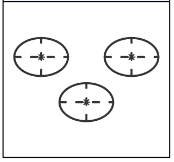
\includegraphics[width=1in, height=0.58in]{./tables/gaussian_param/EEI.png}\\
\midrule
\multicolumn{1}{c}{VEI} & \multicolumn{1}{c}{$[\lambda_j D]$} & \multicolumn{1}{c}{Diagonal} & \multicolumn{1}{c}{IP} & \multicolumn{1}{c}{$\alpha + d + k - 1$} & \multicolumn{1}{c}{}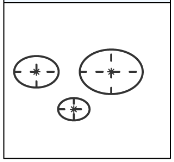
\includegraphics[width=1in, height=0.58in]{./tables/gaussian_param/VEI.png}\\
\midrule
\multicolumn{1}{c}{EVI} & \multicolumn{1}{c}{$[\lambda D_j]$} & \multicolumn{1}{c}{Diagonal} & \multicolumn{1}{c}{CF} & \multicolumn{1}{c}{$\alpha + kd - k + 1$} & \multicolumn{1}{c}{}
\includegraphics[width=1in, height=0.58in]{./tables/gaussian_param/EVI.png}\\
\midrule
\addlinespace
\multicolumn{1}{c}{VVI} & \multicolumn{1}{c}{$[\lambda_j D_j]$} & \multicolumn{1}{c}{Diagonal} & \multicolumn{1}{c}{CF} & \multicolumn{1}{c}{$\alpha + kd$} & \multicolumn{1}{c}{}
\includegraphics[width=1in, height=0.58in]{./tables/gaussian_param/VVI.png}\\
\midrule
\multicolumn{1}{c}{EEE} & \multicolumn{1}{c}{$[\lambda Q D Q^\top]$} & \multicolumn{1}{c}{Ellipsoidal} & \multicolumn{1}{c}{CF} & \multicolumn{1}{c}{$\alpha + \beta$} & \multicolumn{1}{c}{}
\includegraphics[width=1in, height=0.58in]{./tables/gaussian_param/EEE.png}\\
\midrule
\multicolumn{1}{c}{EVE} & \multicolumn{1}{c}{$[\lambda QD_j Q^\top]$} & \multicolumn{1}{c}{Ellipsoidal} & \multicolumn{1}{c}{IP} & \multicolumn{1}{c}{$\alpha + \beta$} & \multicolumn{1}{c}{}
\includegraphics[width=1in, height=0.58in]{./tables/gaussian_param/EVE.png}\\
\midrule
\multicolumn{1}{c}{VEE} & \multicolumn{1}{c}{$[\lambda_j Q D Q^\top]$} & \multicolumn{1}{c}{Ellipsoidal} & \multicolumn{1}{c}{IP} & \multicolumn{1}{c}{$\alpha + \beta + (k-1)(d-1)$} & \multicolumn{1}{c}{}
\includegraphics[width=1in, height=0.58in]{./tables/gaussian_param/VEE.png}\\
\midrule
\multicolumn{1}{c}{VVE} & \multicolumn{1}{c}{$[\lambda_j QD_j Q^\top]$} & \multicolumn{1}{c}{Ellipsoidal} & \multicolumn{1}{c}{IP} & \multicolumn{1}{c}{$\alpha + \beta + d(k-1)$} & \multicolumn{1}{c}{}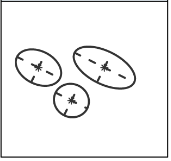
\includegraphics[width=1in, height=0.58in]{./tables/gaussian_param/VVE.png}\\
\midrule
\addlinespace
\multicolumn{1}{c}{EEV} & \multicolumn{1}{c}{$[\lambda Q_j D Q_j^\top]$} & \multicolumn{1}{c}{Ellipsoidal} & \multicolumn{1}{c}{CF} & \multicolumn{1}{c}{$\alpha + k \beta - d(k-1)$} & \multicolumn{1}{c}{}
\includegraphics[width=1in, height=0.58in]{./tables/gaussian_param/EEV.png}\\
\midrule
\multicolumn{1}{c}{VEV} & \multicolumn{1}{c}{$[\lambda_j Q_j D Q_j^\top]$} & \multicolumn{1}{c}{Ellipsoidal} & \multicolumn{1}{c}{IP} & \multicolumn{1}{c}{$\alpha + k \beta - (k-1)(d-1)$} & \multicolumn{1}{c}{}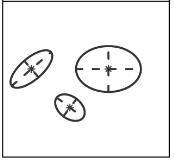
\includegraphics[width=1in, height=0.58in]{./tables/gaussian_param/VEV.png}\\
\midrule
\multicolumn{1}{c}{EVV} & \multicolumn{1}{c}{$[\lambda Q_j D_j Q_j^\top]$} & \multicolumn{1}{c}{Ellipsoidal} & \multicolumn{1}{c}{CF} & \multicolumn{1}{c}{$\alpha + k \beta - k + 1$} & \multicolumn{1}{c}{}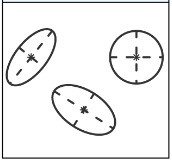
\includegraphics[width=1in, height=0.58in]{./tables/gaussian_param/EVV.png}\\
\midrule
\multicolumn{1}{c}{VVV} & \multicolumn{1}{c}{$[\lambda_j Q_j D_j Q_j^\top]$} & \multicolumn{1}{c}{Ellipsoidal} & \multicolumn{1}{c}{CF} & \multicolumn{1}{c}{$\alpha + k \beta$} & \multicolumn{1}{c}{}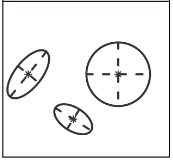
\includegraphics[width=1in, height=0.58in]{./tables/gaussian_param/VVV.png}\\
\midrule
\bottomrule
\end{tabular}}
\end{table}

\hypertarget{references}{%
\section*{References}\label{references}}
\addcontentsline{toc}{section}{References}

\hypertarget{refs}{}
\begin{CSLReferences}{1}{0}
\leavevmode\vadjust pre{\hypertarget{ref-R-EMCluster}{}}%
Chen, Wei-Chen, and Ranjan Maitra. 2022. \emph{EMCluster: EM Algorithm for Model-Based Clustering of Finite Mixture Gaussian Distribution}.

\leavevmode\vadjust pre{\hypertarget{ref-R-bgmm}{}}%
Ewa Szczurek, Przemyslaw Biecek \&. 2021. \emph{Bgmm: Gaussian Mixture Modeling Algorithms and the Belief-Based Mixture Modeling}.

\leavevmode\vadjust pre{\hypertarget{ref-R-mclust}{}}%
Fraley, Chris, Adrian E. Raftery, and Luca Scrucca. 2022. \emph{Mclust: Gaussian Mixture Modelling for Model-Based Clustering, Classification, and Density Estimation}.

\leavevmode\vadjust pre{\hypertarget{ref-R-flexmix}{}}%
Gruen, Bettina, and Friedrich Leisch. 2022. \emph{Flexmix: Flexible Mixture Modeling}.

\leavevmode\vadjust pre{\hypertarget{ref-R-Rmixmod}{}}%
Langrognet, Florent, Remi Lebret, Christian Poli, Serge Iovleff, Benjamin Auder, and Serge Iovleff. 2021. \emph{Rmixmod: Classification with Mixture Modelling}.

\leavevmode\vadjust pre{\hypertarget{ref-R-GMKMcharlie}{}}%
Liu, Charlie Wusuo. 2021. \emph{GMKMcharlie: Unsupervised Gaussian Mixture and Minkowski and Spherical k-Means with Constraints}.

\leavevmode\vadjust pre{\hypertarget{ref-R-mixtools}{}}%
Young, Derek, Tatiana Benaglia, Didier Chauveau, and David Hunter. 2020. \emph{Mixtools: Tools for Analyzing Finite Mixture Models}.

\end{CSLReferences}

\bibliography{RJreferences.bib}

\address{%
Bastien Chassagnol\\
Laboratoire de Probabilités, Statistiques et Modélisation (LPSM), UMR CNRS 8001\\%
4 Place Jussieu Sorbonne Université\\ 75005, Paris, France\\
%
%
\textit{ORCiD: \href{https://orcid.org/0000-0002-8955-2391}{0000-0002-8955-2391}}\\%
\href{mailto:bastien_chassagnol@laposte.net}{\nolinkurl{bastien\_chassagnol@laposte.net}}%
}

\address{%
Antoine Bichat\\
Les Laboratoires Servier\\%
50 Rue Carnot\\ 92150, Suresnes, France\\
%
\url{https://rdrr.io/github/abichat/abutils/}\\%
\textit{ORCiD: \href{https://orcid.org/0000-0001-6599-7081}{0000-0001-6599-7081}}\\%
\href{mailto:antoine.bichat@servier.com}{\nolinkurl{antoine.bichat@servier.com}}%
}

\address{%
Cheïma Boudjeniba\\
Systems Biology Group, Dept. of Computational Biology, Institut Pasteur\\%
25 Rue du Dr Roux\\ 75015 Paris\\
%
%
%
\href{mailto:cheima.boudjeniba@servier.com}{\nolinkurl{cheima.boudjeniba@servier.com}}%
}

\address{%
Pierre-Henri Wuillemin\\
Laboratoire d'Informatique de Paris 6 (LIP6), UMR 7606\\%
4 Place Jussieu Sorbonne Université\\ 75005, Paris, France\\
%
\url{http://www-desir.lip6.fr/~phw/}\\%
\textit{ORCiD: \href{https://orcid.org/0000-0003-3691-4886}{0000-0003-3691-4886}}\\%
\href{mailto:pierre-henri.wuillemin@lip6.fr}{\nolinkurl{pierre-henri.wuillemin@lip6.fr}}%
}

\address{%
Mickaël Guedj\\
Les Laboratoires Servier\\%
50 Rue Carnot\\ 92150, Suresnes, France\\
%
\url{https://michaelguedj.github.io/}\\%
\textit{ORCiD: \href{https://orcid.org/0000-0001-6694-0554}{0000-0001-6694-0554}}\\%
\href{mailto:mickael.guedj@gmail.com}{\nolinkurl{mickael.guedj@gmail.com}}%
}

\address{%
Gregory Nuel\\
Laboratoire de Probabilités, Statistiques et Modélisation (LPSM), UMR CNRS 8001\\%
4 Place Jussieu Sorbonne Université\\ 75005, Paris, France\\
%
\url{http://nuel.perso.math.cnrs.fr/}\\%
\textit{ORCiD: \href{https://orcid.org/0000-0001-9910-2354}{0000-0001-9910-2354}}\\%
\href{mailto:Gregory.Nuel@math.cnrs.fr}{\nolinkurl{Gregory.Nuel@math.cnrs.fr}}%
}

\address{%
Etienne Becht\\
Les Laboratoires Servier\\%
50 Rue Carnot\\ 92150, Suresnes, France\\
%
%
\textit{ORCiD: \href{https://orcid.org/0000-0003-1859-9202}{0000-0003-1859-9202}}\\%
\href{mailto:etienne.becht@servier.com}{\nolinkurl{etienne.becht@servier.com}}%
}

\end{article}


\end{document}
